\subsection{Unregelmäßigkeiten in der Klassifikation des Portals "`BaPVS"'}
    Das Lehrgebiet "`BaPVS"' wurde als erstes auf Basis des
    Klassifizierungsmodells von "`BaBw"' klassifiziert.
    Dabei sind einige neue Auffälligkeiten aufgetreten,
    die in diesem Kapitel beschrieben werden.

    \paragraph{Doppelt klassifizierte Lehrende}
    Drei Mitarbeiter des Portals wurden doppelt klassifiziert.
    Der Grund ist eine abweichende HTML-Struktur,
    die in Listing \ref{listing:findingsTeachersBaPVSHtmlSource} zu sehen ist.

    \lstinputlisting[
        label=listing:findingsTeachersBaPVSHtmlSource,
        caption=Abweichende HTML-Struktur eines Mitarbeiters im Portal BaPVS,
        language=HTML
    ]{../resources/findings/case-study-1/bapvs/teacher.html}

    Im Vergleich zur erwarteten Struktur wiederholt sich
    das div Element mit der Klasse "`grid"',
    weshalb der verwendete Selektor "`section\#content div.grid"'
    betroffene Mitarbeiter doppelt entspricht.

    Für das innere div Element kann das System kein Bild finden,
    weshalb das System zwei Teacher-Knoten anlegt.
    Der erste referenziert ein Bild, der zweite nicht,
    aber beide teilen sich die restlichen Informationen,
    also Name, Lehrgebiet und Kontaktinformationen.
    Dies ist bei zwei Mitarbeitern der Fall.

    Im dritten Fall besitzt der Mitarbeiter kein Bild,
    weshalb der Teacher-Knoten vollständig wiederverwendet werden kann.
    Dennoch enthält die Klassifikation den betroffenen Mitarbeiter zwei Mal.

    \paragraph{Mitarbeiter ohne Lehrgebiet}
    Das Lehrgebiet eines Mitarbeiters wurde vom System nicht erfasst.
    Anders als beim Lehrgebiet "`BaBw"' ist der Grund allerdings,
    dass vor dem Lehrgebiet der Text "`Auskunft erteilt auch:"' platziert ist.
    Der Selektor "`div.team-member-des > p > a:first-child"' findet deshalb
    kein Lehrgebiet, weil er nach einem a Element sucht,
    welches das erste Kindelement seiner Parent Nodes ist.
    Eine naheliegende Lösung ist die Änderung des Selektors,
    sodass er mit "`a:first-of-type"' endet.
    Bei der Erstellung des Klassifizierungsmodells,
    die auf Basis des Portals "`BaBw"' geschah,
    wurde sich allerdings bewusst gegen diese Variante entschieden.
    Bei dem in Kapitel \ref{section:findingsTeachersAbnormalitiesBabw}
    erwähnten Mitarbeiter, für den fälschlicherweise kein Lehrgebiet erkannt wurde,
    hätte dieser Selektor nämlich dazu geführt,
    dass seine E-Mail-Adresse als Lehrgebiet erkannt wird,
    da sie der erste Link ist.

    \paragraph{Falscher Text als Name klassifiziert}
    Als Namen eines Mitarbeiters enthält die Klassifikation
    den Wert "`Auskunft erteilt auch:"'.
    Der Grund ist, dass dieser Text in einem strong-Element steht,
    welches vor dem Namen auftaucht.
    Das System hat in diesem Fall erwartungskonform nur den ersten
    Treffer für das skalare Feature klassifiziert.
        
    \paragraph{28 Mitarbeiter ohne Telefonnummer}
    Einige Kontakte besitzen in der Klassifikation keine Telefonnummer.
    Bei neun ist auch auf der Webseite keine zu finden,
    bei den restlichen ist der Nummer nicht "`Tel.: "'
    sondern "`Telefon: "' oder "`Tel:"' vorangestellt.
    Der Selektor hat deshalb die Nummern nicht erkannt.
    
    \paragraph{56 Mitarbeiter ohne Namen}
    Des Weiteren wurde für eine Vielzahl der Mitarbeiter kein Name erkannt,
    da sie weder in einem strong noch ein einem b Element sind.
    Stattdessen stehen sie wie die Telefonnumer als reiner Text im Element
    oder befinden sich in einem a Element.

    \paragraph{Inkorrekte Telefonnummern}
    Die Klassifikation enthält einige Telefonnummern,
    die neben der eigentlichen Nummer auch weitere Informationen enthalten.
    Ein Beispiel ist "`02331/987-4315 email: Lisa.Schaefer Sprechstunde: nach Vereinbarung via e-mail"'.
    Die Telefonnumer wird über einen XPath-Selektor und der Methode document.evaluate ermittelt,
    die auf dem Quelltext der Webseite agieren.
    Anders als beim Portal "`BaBw"' existieren in "`BaPVS"' Mitarbeiter,
    bei denen die Telefonnumer weder die letzte Angabe ist
    noch von einem Zeilenumbruch gefolgt wird.
    Deshalb wird in diesen Fällen mehr als nur die Telefonnummer ausgewählt.

    \paragraph{Unterschiede im Modell der Seite}
    Im Vergleich zur klassifizierten Seite des Portals "`BaBw"'
    sind auch zwei Unterschiede im Modell der Seite deutlich geworden.
    Der Name eines Mitarbeiters ist in einigen Fällen
    auch ein Link auf eine Detailseite.
    Außerdem besitzen einige Sprechzeiten.

    \paragraph{Falsch annotierte Telefonnummern}
    Bei der Betrachtung der Annotationen im Fall des Portals "`BaBw"'
    ist bereits aufgefallen, dass die Annotation für Telefonnummern
    mehrmals verschoben dargestellt wurde.
    Dies ist im Fall des Portals "`BaPVS"' ebenfalls zu beobachten,
    allerdings in einem deutlicheren Ausmaß,
    wie Abbildung \ref{image:findingTeachersBaPVSWrongPhone} zeigt.

    \begin{figure}[htb]
        \centering
        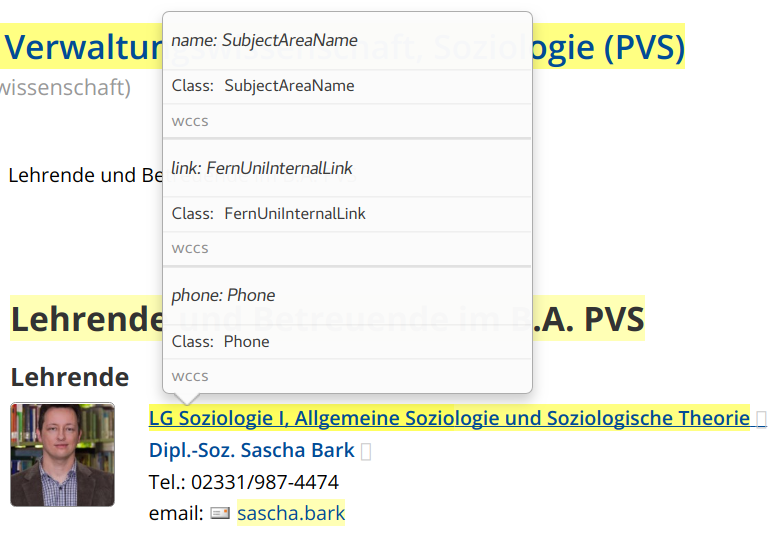
\includegraphics[width=0.5\textwidth]{../resources/findings/case-study-1/bapvs/annotations/triple-annotation.png}
        \caption{Deutlich verschobene Annotation einer Telefonnummer}
        \label{image:findingTeachersBaPVSWrongPhone}
    \end{figure}

    Der Grund steht in Zusammenhang mit der bereits beschriebenen Problematik
    einiger Telefonnummern, die auch andere Informationen enthalten.
    Wie beschrieben befindet sich in diesen Fällen beispielsweise kein
    Zeilenumbruch zwischen Telefonnumer und E-Mail.
    Zur Ermittlung des Startoffsets des eindeutigen Selektors
    wird auf der Eigenschaft "`innerText"' des Parent Nodes
    die Methode "`indexOf"' aufgerufen, der der klassifizierte Text
    übergeben wird. So kann die Position des Textes im Node ermittelt werden.
    Der klassifizierte Text wurde in diesem Fall aber direkt durch den
    XPath-Ausdruck ermittelt.
    D.h. der Ausdruck hat keinen Node geliefert, auf dem das System .innerText
    aufgerufen hat, um den Text zu ermitteln.
    Der vom Ausdruck ermittelte Text basiert aber auf dem Quelltext,
    weshalb HTML-Nodes nicht gerendert werden.
    Im Quelltext steht zwischen Telefonnummer und E-Mail ein br-Tag
    (siehe Listing \ref{listing:findingsTeachersHtmlSource}).
    Die Eigenschaft innerText hat deshalb einen Zeilenumbruch zwischen den beiden.
    Der aus dem Quelltext gewonnene Text aber nicht,
    weshalb indexOf keinen Treffer findet und -1 zurückgibt.
    Die Annotation wird von Annotator deshalb ganz an den Anfang verschoben.